% id: 89-03
% book: 쎈B 대수 · 07 삼각함수의 활용
% section: 유형 01 사인법칙
% figure: tikz:fig-89-03
% answer: 
% answer_source: 
% variant_level: 0 (원본 전사)
% 이 파일은 build.mjs 가 items.json 에서 만든다. 고칠 때는 items.json 을 고친다.
\smash{\raisebox{1.5mm}{\dmkichul{쎈B 대수 89쪽 03번}}}
\noindent\begin{minipage}[t]{0.58\linewidth}\vspace{0pt}\raggedright 오른쪽 그림과 같이 원 위의 네 점 $\pt{A}$, $\pt{B}$, $\pt{C}$, $\pt{D}$에 대하여 $\angle\pt{BAC}=60^\circ$, $\angle\pt{BAD}=90^\circ$이고 $\seg{AB}=\seg{AD}=8$일 때, $\seg{CD}$의 길이를 구하시오.\end{minipage}\hfill\begin{minipage}[t]{0.4\linewidth}\vspace{0pt}\centering \resizebox{\ifdim\width>\linewidth\linewidth\else\width\fi}{!}{% 89-03(89쪽) — 원 위의 네 점 A·B·C·D 와 현 AB·AD·AC·BD·DC(원문 「오른쪽 그림」). 스캔 화질이 낮아 TikZ 로 다시 그림.
% 라벨은 원문 것만 — 네 점 이름, 길이 $8$ 두 개, $\angle\pt{BAC}=60^\circ$, $\angle\pt{BAD}$ 의 직각 표시.
% $\seg{CD}$(답)의 길이는 적지 않는다.
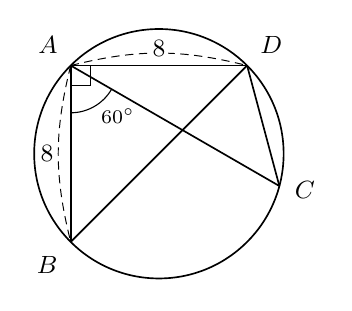
\begin{tikzpicture}[line width=0.6pt]
  \coordinate (A) at (0,2.24);
  \coordinate (B) at (0,0);
  \coordinate (C) at (2.650,0.710);
  \coordinate (D) at (2.24,2.24);
  \draw (1.12,1.12) circle (1.584);
  \draw (A) -- (D);
  \draw (A) -- (B);
  \draw (A) -- (C);
  \draw (B) -- (D);
  \draw (D) -- (C);
  % 직각 표시 $\angle\pt{BAD}$
  \draw[line width=0.4pt] (0,1.99) -- (0.25,1.99) -- (0.25,2.24);
  % $60^\circ$ = $\angle\pt{BAC}$
  \draw[line width=0.4pt] (0,1.64) arc (270:330:0.6);
  \node[font=\scriptsize] at (0.60,1.60) {$60^\circ$};
  % 길이 표시의 점선 호
  \draw[densely dashed, line width=0.35pt] (A) to[bend left=14] (D);
  \draw[densely dashed, line width=0.35pt] (A) to[bend right=14] (B);
  \node[font=\small, fill=white, inner sep=1pt] at (1.12,2.46) {$8$};
  \node[font=\small, fill=white, inner sep=1pt] at (-0.30,1.12) {$8$};
  \node[font=\small, anchor=south east] at (-0.04,2.26) {$\pt{A}$};
  \node[font=\small, anchor=north east] at (-0.04,-0.06) {$\pt{B}$};
  \node[font=\small, anchor=west] at (2.72,0.66) {$\pt{C}$};
  \node[font=\small, anchor=south west] at (2.28,2.26) {$\pt{D}$};
\end{tikzpicture}
}\end{minipage}\par
